%%%%%%%%%%%%%%%%%%%%%%%%%%%%%%%%%%%%%%%%%%%
%
% From a template maintained at https://github.com/jamesrobertlloyd/cbl-tikz-poster
%
% Code near the top should be fairly standard and not need to be changed
%  - except for the document class
% Code lower down is more likely to be customised
%
%%%%%%%%%%%%%%%%%%%%%%%%%%%%%%%%%%%%%%%%%%%


\documentclass[landscape,a0b,final,a4resizeable]{include/a0poster}
\usepackage[utf8]{inputenc}

\usepackage{multicol}
\usepackage{color}
\usepackage{morefloats}
\usepackage[pdftex]{graphicx}
\usepackage{rotating}
\usepackage{amsmath, amsthm, amssymb, bm}
\usepackage{array}
\usepackage{booktabs}
\usepackage{multirow}
\usepackage{hyperref}
\usepackage[margin=30mm, bottom=40mm]{geometry}
\usepackage{rotating}

\usepackage{include/picins}
\usepackage{tikz}
\usetikzlibrary{shapes.geometric,arrows,chains,matrix,positioning,scopes,calc}
\tikzstyle{mybox} = [draw=white, rectangle]
\definecolor{darkblue}{rgb}{0,0.08,0.45}
\definecolor{blue}{rgb}{0,0,1}

\usepackage{dsfont}

%%%%%%%%%%%%%%%%%%%%%%%%%%%%%%%%%%%%%%%%%%%
%
% myfig
%
% \myfig - replacement for \figure
% necessary, since in multicol-environment 
% \figure won't work        
%                 
%%%%%%%%%%%%%%%%%%%%%%%%%%%%%%%%%%%%%%%%%%%

\newcommand{\myfig}[3][0]{
\begin{center}
  \vspace{1.5cm}
  \includegraphics[width=#3\hsize,angle=#1]{#2}
  \nobreak\medskip
\end{center}}

%%%%%%%%%%%%%%%%%%%%%%%%%%%%%%%%%%%%%%%%%%%
%
% mycaption                
%
% \mycaption - replacement for \caption
% necessary, since in multicol-environment \figure and
% therefore \caption won't work
%
%%%%%%%%%%%%%%%%%%%%%%%%%%%%%%%%%%%%%%%%%%%

%\newcounter{figure}
\setcounter{figure}{1}
\newcommand{\mycaption}[1]{
  \vspace{0.5cm}
  \begin{quote}
    {{\sc Figure} \arabic{figure}: #1}
  \end{quote}
  \vspace{1cm}
  \stepcounter{figure}
}

%%%%%%%%%%%%%%%%%%%%%%%%%%%%%%%%%%%%%%%%%%%
%
% Some standard colours
%
%%%%%%%%%%%%%%%%%%%%%%%%%%%%%%%%%%%%%%%%%%%

\definecolor{camlightblue}{rgb}{0.601 , 0.8, 1}
\definecolor{camdarkblue}{rgb}{0, 0.203, 0.402}
\definecolor{camred}{rgb}{1, 0.203, 0}
\definecolor{camyellow}{rgb}{1, 0.8, 0}
\definecolor{lightblue}{rgb}{0, 0, 0.80}
\definecolor{white}{rgb}{1, 1, 1}
\definecolor{whiteblue}{rgb}{0.80, 0.80, 1}

%%%%%%%%%%%%%%%%%%%%%%%%%%%%%%%%%%%%%%%%%%%
%
% Some look and feel definitions
%
%%%%%%%%%%%%%%%%%%%%%%%%%%%%%%%%%%%%%%%%%%%

\setlength{\columnsep}{0.03\textwidth}
\setlength{\columnseprule}{0.0018\textwidth}
\setlength{\parindent}{0.0cm}

%%%%%%%%%%%%%%%%%%%%%%%%%%%%%%%%%%%%%%%%%%%
%
% \mysection - replacement for \section*
% 
% Puts a pretty box around some text
% TODO - any other thoughts for what this box should look like
%
%%%%%%%%%%%%%%%%%%%%%%%%%%%%%%%%%%%%%%%%%%%

\tikzstyle{mysection} = [rectangle, 
			draw=none, 
			shade, 
			outer color=camlightblue!00,
			inner color=camlightblue!00,
			text width=0.965\columnwidth,
			text centered,
			rounded corners=20pt,
			minimum height=0.09\columnwidth]

\newcommand{\mysection}[1]
{
\begin{center}
  \begin{tikzpicture}
    \node[mysection] {\sffamily\bfseries\huge#1};
  \end{tikzpicture}
\end{center}
}

%%%%%%%%%%%%%%%%%%%%%%%%%%%%%%%%%%%%%%%%%%%
%
% Set the font
%
% TODO - Not sure what a canonical choice is - feel free to modify
%
%%%%%%%%%%%%%%%%%%%%%%%%%%%%%%%%%%%%%%%%%%%

\renewcommand{\familydefault}{cmss}
\sffamily

%%%%%%%%%%%%%%%%%%%%%%%%%%%%%%%%%%%%%%%%%%%%%%%%%%%%
%%%               Background                     %%%
%%%%%%%%%%%%%%%%%%%%%%%%%%%%%%%%%%%%%%%%%%%%%%%%%%%%

\newcommand{\background}[3]{
  %\definecolor{cgradbegin}{#1}
  %\definecolor{cgradend}{#2}
 % \psframe[fillstyle=gradient,gradend=cgradend,
 % gradbegin=cgradbegin,gradmidpoint=#3](0.,0.)(1.\textwidth,-1.\textheight)
}




%%%%%%%%%%%%%%%%%%%%%%%%%%%%%%%%%%%%%%%%%%%%%%%%%%%%
%%%                pcolumn                       %%%
%%%%%%%%%%%%%%%%%%%%%%%%%%%%%%%%%%%%%%%%%%%%%%%%%%%%

\newenvironment{pcolumn}[1]{
  \begin{minipage}{#1\textwidth}
  \begin{center}
}{
  \end{center}
  \end{minipage}
}



%%%%%%%%%%%%%%%%%%%%%%%%%%%%%%%%%%%%%%%%%%%%%%%%%%%%
%%%                pbox                          %%%
%%%%%%%%%%%%%%%%%%%%%%%%%%%%%%%%%%%%%%%%%%%%%%%%%%%%

\definecolor{lcolor}{rgb}{0, 0, 0.80}
\definecolor{gcolor1}{rgb}{1, 1, 1}
\definecolor{gcolor2}{rgb}{.80, .80, 1}

  % \def\fc{fillcolor}
  % \def\getfc #1=#2\par{\def\ffc{#1} \ifx\ffc\fc #2\fi} 
  % \def\getfillcolor #1,#2\par{\getfc #1\par \getfc #2\par}

 %  \newcommand{\psshadowbox}[2]{%[2][magenta]{
%      \fbox{Input arg: #1}
%      \fbox{#1} 
%      \fbox {\getfillcolor #1\par}
%      \def\col{\getfillcolor #1\par}
 
%      \let\coll=\col
%       \coll
 %     \colorbox{\col}{#2}
%       \mbox
   %   \coloredshadowbox{black}{\coll}{#2}
%   }

\newcommand{\pbox}[4]{
%\psshadowbox[#3]{
%\fbox{
\mbox{
\begin{minipage}[t][#2][t]{#1}
#4
\end{minipage}
}%}
}

%%%%%%%%%%%%%%%%%%%%%%%%%%%%%%%%%%%%%%%%%%%
%
% Poster environment
%
% Centres everything and can be used to define the width of the content
%
%%%%%%%%%%%%%%%%%%%%%%%%%%%%%%%%%%%%%%%%%%%

\newenvironment{poster}{
  \begin{center}
  \begin{minipage}[c]{\textwidth}
}{
  \end{minipage}
  \end{center}
}

\def\newarrow{\mbox{\begin{tikzpicture}
             \useasboundingbox{(-3pt,-4.5pt) rectangle (19pt,1pt)};
             \draw[->] (0,-0.07)--(17pt,-0.07);\end{tikzpicture}}}



\ProvidesPackage{preamble}

\usepackage{url}
\usepackage{array}
\usepackage{amsmath,amssymb,amsfonts,textcomp}
\usepackage{booktabs}
\usepackage{relsize}
\usepackage{nicefrac}
\usepackage{graphicx}
\usepackage{rotating}
\usepackage{nth}
\usepackage{acronym}
\usepackage{bm}

\newcommand{\binarysum}{\sum_{\bf{x} \in \{0,1\}^D}}
\newcommand{\expect}{\mathbb{E}}
\newcommand{\expectargs}[2]{\mathbb{E}_{#1} \left[ {#2} \right]}
\newcommand{\var}{\mathbb{V}}
\newcommand{\varianceargs}[2]{\mathbb{V}_{#1} \left[ {#2} \right]}
\newcommand{\variance}{\mathbb{V}}
\newcommand{\cov}{\operatorname{cov}}
\newcommand{\Cov}{\operatorname{Cov}}
\newcommand{\covarianceargs}[2]{\Cov_{#1} \left[ {#2} \right]}
\newcommand{\colvec}[2]{\left[ \begin{array}{c} {#1} \\ {#2} \end{array} \right]}
\newcommand{\tbtmat}[4]{\left[ \begin{array}{cc} {#1} & {#2} \\ {#3} & {#4} \end{array} \right]}

%\newcommand{\covskinny}[2]{\var\!\left(#1\middle\vert#2\right)} 

\newcommand{\acro}[1]{\textsc{#1}}
%\newcommand{\vect}[1]{\boldsymbol{#1}}
\newcommand{\vect}[1]{{\bf{#1}}}
\newcommand{\mat}[1]{\mathbf{#1}}
\newcommand{\pderiv}[2]{\frac{\partial #1}{\partial #2}}
\newcommand{\npderiv}[2]{\nicefrac{\partial #1}{\partial #2}}

\newcommand{\pha}{^{\phantom{:}}}

\newcommand{\argmin}{\operatornamewithlimits{argmin}}
\newcommand{\argmax}{\operatornamewithlimits{argmax}}

% The following designed for probabilities with long arguments

\newcommand{\Prob}[2]{P\!\left(\,#1\;\middle\vert\;#2\,\right)}
\newcommand{\ProbF}[3]{P\!\left(\,#1\!=\!#2\;\middle\vert\;#3\,\right)}
\newcommand{\p}[2]{p\!\left(#1\middle\vert#2\right)}
\newcommand{\po}[1]{p\!\left(#1\right)}
\newcommand{\pF}[3]{p\!\left(\,#1\!=\!#2\;\middle\vert\;#3\,\right)} 
\newcommand{\mean}[2]{{m}\!\left(#1\middle\vert#2\right)}
%\newcommand{\novmean}[2]{{m}\!\left(#1\middle\vert#2\right)}
%\newcommand{\novcov}[2]{\var\!\left(#1\middle\vert#2\right)}
%\newcommand{\cov}[2]{\var\!\left(#1\middle\vert#2\right)} 
%\newcommand{\pskinny}[2]{p\!\left(#1\;\middle\vert\;#2\right)}
%\newcommand{\meanskinny}[2]{{m}\!\left(#1\middle\vert#2\right)}
%\newcommand{\covskinny}[2]{\var\!\left(#1\middle\vert#2\right)} 

\newcommand{\vI}{\mat{I}}
\newcommand{\vX}{\mat{X}}
\newcommand{\vY}{\mat{Y}}
\newcommand{\vZ}{\mat{Z}}
\newcommand{\vK}{\mat{K}}
\newcommand{\vs}{\vect{s}}
\newcommand{\va}{\vect{a}}
\newcommand{\vA}{\vect{A}}
\newcommand{\vb}{\vect{b}}
\newcommand{\vB}{\mat{B}}
\newcommand{\vR}{\mat{R}}
\newcommand{\vS}{\mat{S}}
\newcommand{\vu}{\vect{u}}
\newcommand{\vk}{\vect{k}}
\newcommand{\vc}{\vect{c}}
\newcommand{\vC}{\mat{C}}
\newcommand{\vw}{\vect{w}}
\newcommand{\vx}{\vect{x}}
\newcommand{\vy}{\vect{y}}
\newcommand{\vz}{\vect{z}}
\newcommand{\vmu}{\vect{\mu}}
\newcommand{\vpi}{\vect{\pi}}
\newcommand{\vphi}{\vect{\phi}}
\newcommand{\vSigma}{\mat{\Sigma}}
\newcommand{\vtheta}{\vect{\theta}}
\newcommand{\vl}{\vect{l}}
\newcommand{\vq}{\vect{q}}
\newcommand{\vf}{\vect{f}}
\newcommand{\vg}{\vect{g}}
\newcommand{\vell}{\vect{\ell}}
\newcommand{\ve}{\vect{\epsilon}}
\newcommand{\vzero}{\vect{0}}
\newcommand{\vone}{\vect{1}}

\newcommand{\He}{\mathcal{H}}
\newcommand{\normx}[2]{\left\|#1\right\|_{#2}}
\newcommand{\Hnorm}[1]{\normx{#1}{\He}}
\newcommand{\mmd}{{\rm MMD}}


\newcommand{\mf}{\bar{\vf}}

\newcommand{\st}{_\star}

\newcommand{\inv}{^{{\mathsmaller{-1}}}}
\newcommand{\tohalf}{^{{\mathsmaller{\nicefrac{1}{2}}}}}

\newcommand{\N}[3]{\mathcal{N}\!\left(#1|#2,#3\right)}
\newcommand{\bN}[3]{\mathcal{N}\big(#1|#2,#3\big)}
\newcommand{\boldN}[3]{\text{\textbf{\mathcal{N}}}\big(#1;#2,#3\big)}
\newcommand{\ones}[1]{\mat{1}_{#1}}
\newcommand{\eye}[1]{\mat{E}_{#1}}
\newcommand{\tra}{^\ensuremath{\mathsf{T}}}
\newcommand{\trace}{\operatorname{tr}}
\newcommand{\deq}{:=}
\newcommand{\degree}{^\circ}

\DeclareMathOperator{\chol}{chol}
\DeclareMathOperator{\diag}{diag}

\newcommand{\gp}{{\acro{gp}}}
\newcommand{\bmc}{{\acro{bmc}}}
\newcommand{\bq}{{\acro{bq}}}
\newcommand{\sbq}{{\acro{sbq}}}

\newenvironment{narrow}[2]{%
  \begin{list}{}{%
  \setlength{\topsep}{0pt}%
  \setlength{\leftmargin}{#1}%
  \setlength{\rightmargin}{#2}%
  \setlength{\listparindent}{\parindent}%
  \setlength{\itemindent}{\parindent}%
  \setlength{\parsep}{\parskip}}%
\item[]}{\end{list}}

\newtheorem{prop}{Proposition}
\newtheorem{cor}{Corollary}
\newtheorem{lem}{Lemma}


\def\ie{i.e.\ }
\def\eg{e.g.\ }
\def\iid{i.i.d.\ }
\def\simiid{\sim_{\mbox{\tiny iid}}}
\def\eqdist{\stackrel{\mbox{\tiny d}}{=}}

\def\Reals{\mathbb{R}}

\def\Uniform{\mbox{\rm Uniform}}
\def\Bernoulli{\mbox{\rm Bernoulli}}
\def\GP{\mathcal{GP}}

\def\inputVar{x}
\def\InputVar{X}
\def\InputSpace{\mathcal{X}}
\def\outputVar{y}
\def\OutputSpace{\mathcal{Y}}
\def\function{f}
\def\kernel{k}
\def\KernelMatrix{K}
\def\SumKernel{\sum}
\def\ProductKernel{\prod}
\def\expression{e}

\def\SE{\acro{SE}}
\def\Per{\acro{Per}}
\def\RQ{\acro{RQ}}
\def\Lin{\acro{Lin}}

\def\subexpr{{\cal S}}
\def\baseker{{\cal B}}
\def\numWinners{k}

\newcommand{\kSE}{{\acro{SE}}}
\newcommand{\kC}{{\acro{C}}}
\newcommand{\kPer}{{\acro{Per}}}
\newcommand{\kLin}{{\acro{Lin}}}
\newcommand{\kWN}{{\acro{WN}}}
\newcommand{\kCP}{{\acro{CP}}}
\newcommand{\kCW}{{\acro{CW}}}
\newcommand{\kRQ}{{\acro{RQ}}}

\newcommand{\vv}{\mathbf{v}}

% Basic function commands.
\newcommand{\Func}[2]{#1 \left( #2\right)}
\newcommand{\FuncSq}[2]{#1 \left[ #2 \right]}
\newcommand{\CondFunc}[3]{#1 \left(#2 \, \middle\vert \, #3 \right)}
\newcommand{\pProb}[1]{\Func{p}{#1}}
\newcommand{\ProbC}[2]{\Func{p_{#1}}{#2}}
\newcommand{\Cond}[2]{\CondFunc{p}{#1}{#2}}
\newcommand{\CondC}[3]{\CondFunc{p_{#1}}{#2}{#3}}

% Distributions.
\newcommand{\dNorm}[1]{\Func{\textrm{N}}{#1}}
\newcommand{\dDir}[1]{\Func{\textrm{Dir}}{#1}}
\newcommand{\dNIW}[1]{\Func{\textrm{NIW}}{#1}}
\newcommand{\dIW}[1]{\Func{\textrm{IW}}{#1}}
\newcommand{\dGam}[1]{\Func{\textrm{G}}{#1}}
\newcommand{\dNG}[1]{\Func{\textrm{NG}}{#1}}
\newcommand{\dBern}[1]{\Func{\textrm{Bernoulli}}{#1}}
\newcommand{\dCat}[1]{\Func{\textrm{Cat}}{#1}}
\newcommand{\dInvGam}[1]{\Func{\textrm{G}^{-1}}{#1}}
\newcommand{\dDirMulti}[1]{\Func{\textrm{DirMulti}}{#1}}
\newcommand{\dT}[1]{\Func{\textrm{T}}{#1}}
\newcommand{\dUnif}[1]{\textrm{Unif}{#1}}

% Probability density / mass functions.
\newcommand{\pdfNorm}[2]{\CondFunc{\textrm{N}}{#1}{#2}}
\newcommand{\pdfDir}[2]{\CondFunc{\textrm{Dir}}{#1}{#2}}
\newcommand{\pdfNIW}[2]{\CondFunc{\textrm{NIW}}{#1}{#2}}
\newcommand{\pdfIW}[2]{\CondFunc{\textrm{IW}}{#1}{#2}}
\newcommand{\pdfGam}[2]{\CondFunc{\textrm{G}}{#1}{#2}}
\newcommand{\pdfNG}[2]{\CondFunc{\textrm{NG}}{#1}{#2}}
\newcommand{\pdfCat}[2]{\CondFunc{\textrm{Cat}}{#1}{#2}}
\newcommand{\pdfInvGam}[2]{\CondFunc{\textrm{G}^{-1}}{#1}{#2}}
\newcommand{\pdfDirMulti}[2]{\CondFunc{\textrm{DirMulti}}{#1}{#2}}
\newcommand{\pdfT}[2]{\CondFunc{\textrm{T}}{#1}{#2}}

% Normalising constants.
\newcommand{\ZDir}[1]{\Func{Z_{\textrm{Dir}}}{#1}}

% Misc functions.
\renewcommand{\det}[1]{\left| #1 \right|}
\newcommand{\Log}[1] {\Func{\textrm{log}}{#1}}
\newcommand{\MvGamma}[2]{\Func{\Gamma_{#1}}{#2}}
\newcommand{\Indic}[1]{\Func{\mathbb{I}}{#1}}
\newcommand{\Expect}[2]{\FuncSq{\mathbb{E}_{#1}}{#2}}
\newcommand{\DivKL}[2]{\Func{\textrm{D}_{KL}}{#1 \, \mid \mid \, #2}}
\newcommand{\GammaFunc}[1]{\Func{\Gamma}{#1}}

% Miscellaneous symbols used regularly throughout.
\newcommand{\xbar}{\overline{\mathbf{x}}}
\newcommand{\xbarl}{\overline{x}}
\newcommand{\Simp}[1]{\mathcal{S}^{#1}}

\usetikzlibrary{fit,positioning}

\vspace{0.5in}

\begin{document}
\begin{poster} 

% Potentially add some space at the top of the poster
\vspace{0\baselineskip}


%%% Header
\begin{center}
\begin{pcolumn}{0.99}

\newcommand{\logowidth}{0.11\textwidth}

\pbox{0.99\textwidth}{}{linewidth=2mm,framearc=0.3,linecolor=camdarkblue,fillstyle=gradient,gradangle=0,gradbegin=white,gradend=white,gradmidpoint=1.0,framesep=1em}{
%
%%% Cambridge Logo
\begin{minipage}[c]{\logowidth}
  \begin{center}
    
\includegraphics[width=5cm]{badges/cambridgecrest}
  \end{center}
\end{minipage}
%
%%% Title
\begin{minipage}[c][9cm][c]{0.76\textwidth}
  \begin{center}
    {\sffamily \VeryHuge \textbf{Auto-Encoding Variational Bayes}}\\[10mm]
    {\huge\sffamily \Huge Paweł F. P. Budzianowski, Thomas F. W. Nicholson, William C. Tebbutt \\[7.5mm]
    %\texttt{\{ti242, dkd23, zoubin\}@cam.ac.uk}
    }
  \end{center}
\end{minipage}
%
%
% Harvard logo
\begin{minipage}[c]{\logowidth}
  \begin{flushright}
    
\includegraphics[width=15cm, clip]{badges/camtext}
  \end{flushright}
\end{minipage}
%
}
\end{pcolumn}
\end{center}

\vspace*{3cm}

\Large


%%%%%%%%%%%%%%%%%%%%%%%%%%%%%%%%%%%%%%%%%%%%%%%%%%%%%%%%%%%%%%%%%%%%%%
%%% Beginning of Document
%%%%%%%%%%%%%%%%%%%%%%%%%%%%%%%%%%%%%%%%%%%%%%%%%%%%%%%%%%%%%%%%%%%%%%


\begin{multicols}{3}

\mysection{Problem Definition}
\vspace{0.25in}
Perform approximate inference in model with local latent variables $z_i$ whilst learning point estimates for the MAP solution for the global parameters $\theta$ having observed $x_i$.

\vspace{0.5in}

\begin{center}
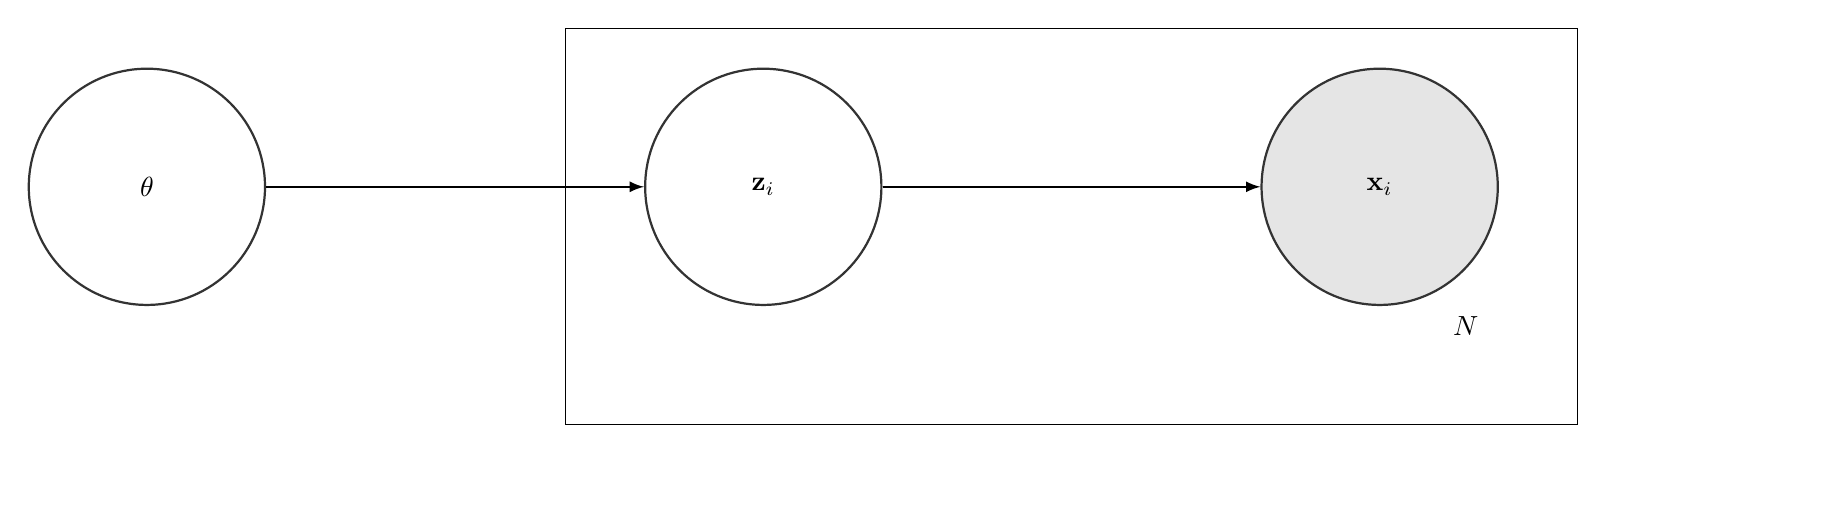
\begin{tikzpicture}
\tikzstyle{main}=[circle, minimum size = 30mm, thick, draw =black!80, node distance = 48mm]
\tikzstyle{connect}=[-latex, thick]
\tikzstyle{box}=[rectangle, draw=black!100]
  \node[main, fill = white!100] (theta) {$\theta$};
  \node[main, fill = white!100, right=of theta] (C1) {$\mathbf{z}_i$};
  \node[main, fill = black!10, right=of C1] (X1) {$\mathbf{x}_i$};
  \path (theta) edge [connect] (C1)
        (C1) edge [connect] (X1);
  \node[rectangle, inner sep=0mm, fit= (C1) (X1),label=below right:$N$, yshift=0mm, xshift=32mm] {};
  \node[rectangle, inner sep=10mm,draw=black!100, fit= (C1) (X1), yshift=-5mm] {};
  \path
    ([shift={(50\pgflinewidth,-50\pgflinewidth)}]current bounding box.south west)
    ([shift={( 50\pgflinewidth, -150\pgflinewidth)}]current bounding box.north east);
\end{tikzpicture}
\end{center}

%\vspace{-0.5in}

\vspace{0.5in}

\mysection{SGVB}

Stochastic Gradient Variational Bayes provides a method to find a deterministic approximation to an intractable posterior distribution by finding parameters $\phi$ such that $\DivKL{\CondFunc{q_\phi}{\mathbf{z}_i}{\mathbf{x}_i}}{\CondFunc{p_\theta}{\mathbf{z}_i}{\mathbf{x}_i}}$ is minimised for all $i$. This is achieved by, for each observation, maximising a lower bound
\begin{equation}
  \Func{\mathcal{L}}{\phi; \mathbf{x}_i} = \Expect{\CondFunc{q_\phi}{\mathbf{z}_i}{\mathbf{x}_i}}{\log \CondFunc{p_\theta}{\mathbf{z}_i}{\mathbf{x}_i}} - \DivKL{\CondFunc{q_\phi}{\mathbf{z}_i}{\mathbf{x}_i}}{\pProb{\mathbf{z}_i}}. \nonumber 
\end{equation}
The expectation term in this lower bound cannot typically be computed exactly.
\begin{align}
  \Func{\tilde{\mathcal{L}}^B}{\theta, \phi; \mathbf{x}_i} = \frac{1}{L} \sum_{l=1}^{L} \log \CondFunc{p_\theta}{\mathbf{x}_i}{\mathbf{z}_{i,l}} - \DivKL{\CondFunc{q_{\phi}}{\mathbf{z}_i}{\mathbf{x}_i}}{\Func{p_\theta}{\mathbf{z}_i}}, \nonumber 
\end{align}
where reparameterising $\mathbf{\mathbf{z}}$ = $g_\phi(\mathbf{x}, \mathbf{\epsilon})$ with  $\mathbf{\epsilon} \sim p(\mathbf{\epsilon})$ yields a differentiable Monte Carlo approximation.

\vspace{0.5in}

\mysection{Variational Autoencoder}
The Variational Autoencoder is a generative latent variable model for data in which $\mathbf{z}_i \sim \mathcal{N}(\mathbf{0}, \mathbf{I})$ and $\mathbf{x}_i \sim \CondFunc{p_\theta}{\mathbf{x}_i}{\mathbf{z}_i}$, where this conditional is parameterised by an multi-layer perceptron (MLP).\\

An MLP recognition model $\CondFunc{q_\phi}{\mathbf{z}_i}{\mathbf{x}_i}$ is used to provide fast approximate posterior inference in $\mathbf{z}_i \mid \mathbf{x}_i$.\\

The MLPs used in the recognition model $q_\phi$ and conditional distribution $\CondFunc{p_\theta}{\mathbf{x}_i}{\mathbf{z}_i}$ are often compared to the encoder and decoder networks in traditional autoencoders respectively.



\newpage %%%%%%%%%%%%%%%%%%%%%%%%%%%%%%%%%%%%%%%%%%%%%%%%%%%%%%%%%%%%%%%%%%%%%%%%%%%%%%%%%%%%%%%%%%%%%%%


\mysection{Noisy KL-divergence estimate}
In the case of the non-Gaussian distributions, it is often impossible to obtain closed-form expression for the KL-divergence term which also requires estimation by sampling. This yields more generic estimator of the form:
$$ \widetilde{\mathcal{L}}^{A}(\theta, \boldsymbol{\phi}; \mathbf{x}^{(i)}) = \frac{1}{L} \sum_{l=1}^L \left( \log p_{\theta}(\mathbf{x}^{(i)}, \mathbf{z}^{(i,l)}) - \log q_{\phi}(\mathbf{z}^{(i,l)} | \mathbf{x}^{(i)} \right).$$

\vspace{0.5em}

\begin{center}
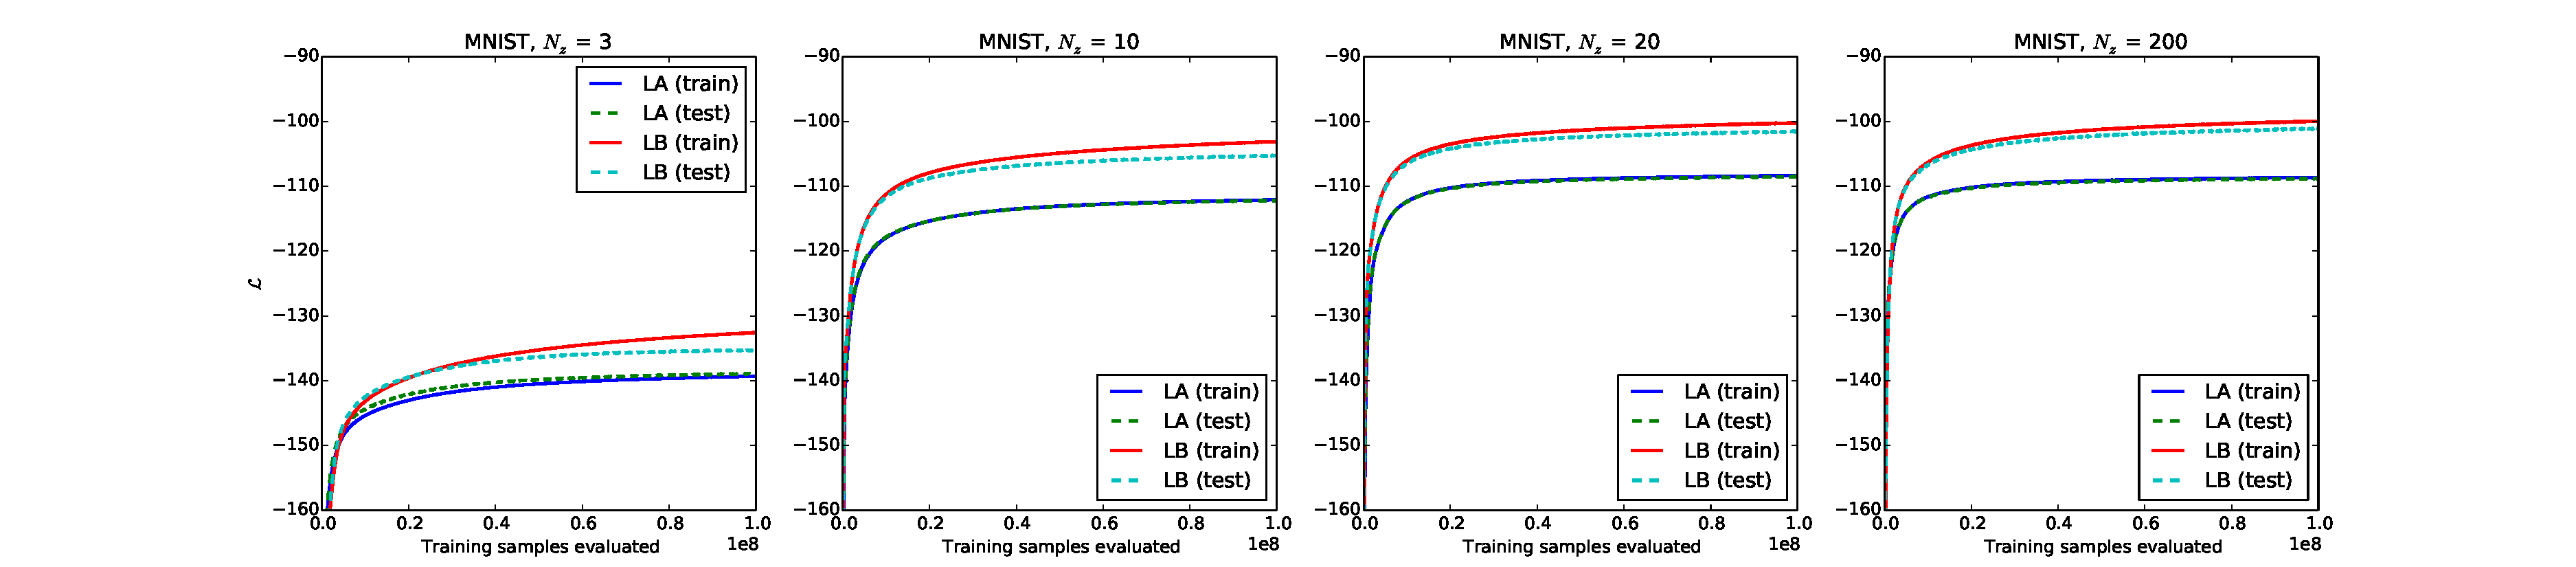
\includegraphics[width=1\columnwidth]{../res/mnist_LAvsLB}
\end{center}

\vspace{0.5em}

\mysection{Visualisation of learned manifolds}

The linearly spaced grid of coordinates over the unit square is mapped through the inverse CDF of the Gaussian to obtain the value of $\mathbf{z}$ which can be used to sample from $p_{\mathbf{\theta}} (\mathbf{x}| \mathbf{z})$ with the estimated parameters $\boldsymbol{\theta}$.

\vspace{0.5em}

\begin{tabular}{cc}
\begin{minipage}[c]{0.48\columnwidth}
\hspace{2em}
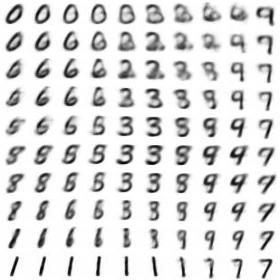
\includegraphics[width=.6\columnwidth]{../freyFaces/MNIST}
\end{minipage} & 
\begin{minipage}[c]{0.48\columnwidth}
\begin{center}
\vspace{0.5cm}
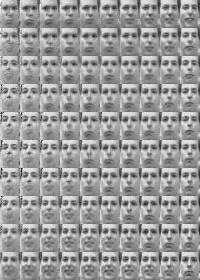
\includegraphics[width=.5\columnwidth]{../freyFaces/FREY}
\end{center}
\end{minipage}
\end{tabular}

\vspace{0.5em}

\mysection{Bayesian: is it really all that?}
Comparing reconstruction error to vanilla auto-encoder, we see stronger performance from VAEB.

\begin{tabular}{cc}
\begin{minipage}[c]{0.5\columnwidth}
\hspace{0em}
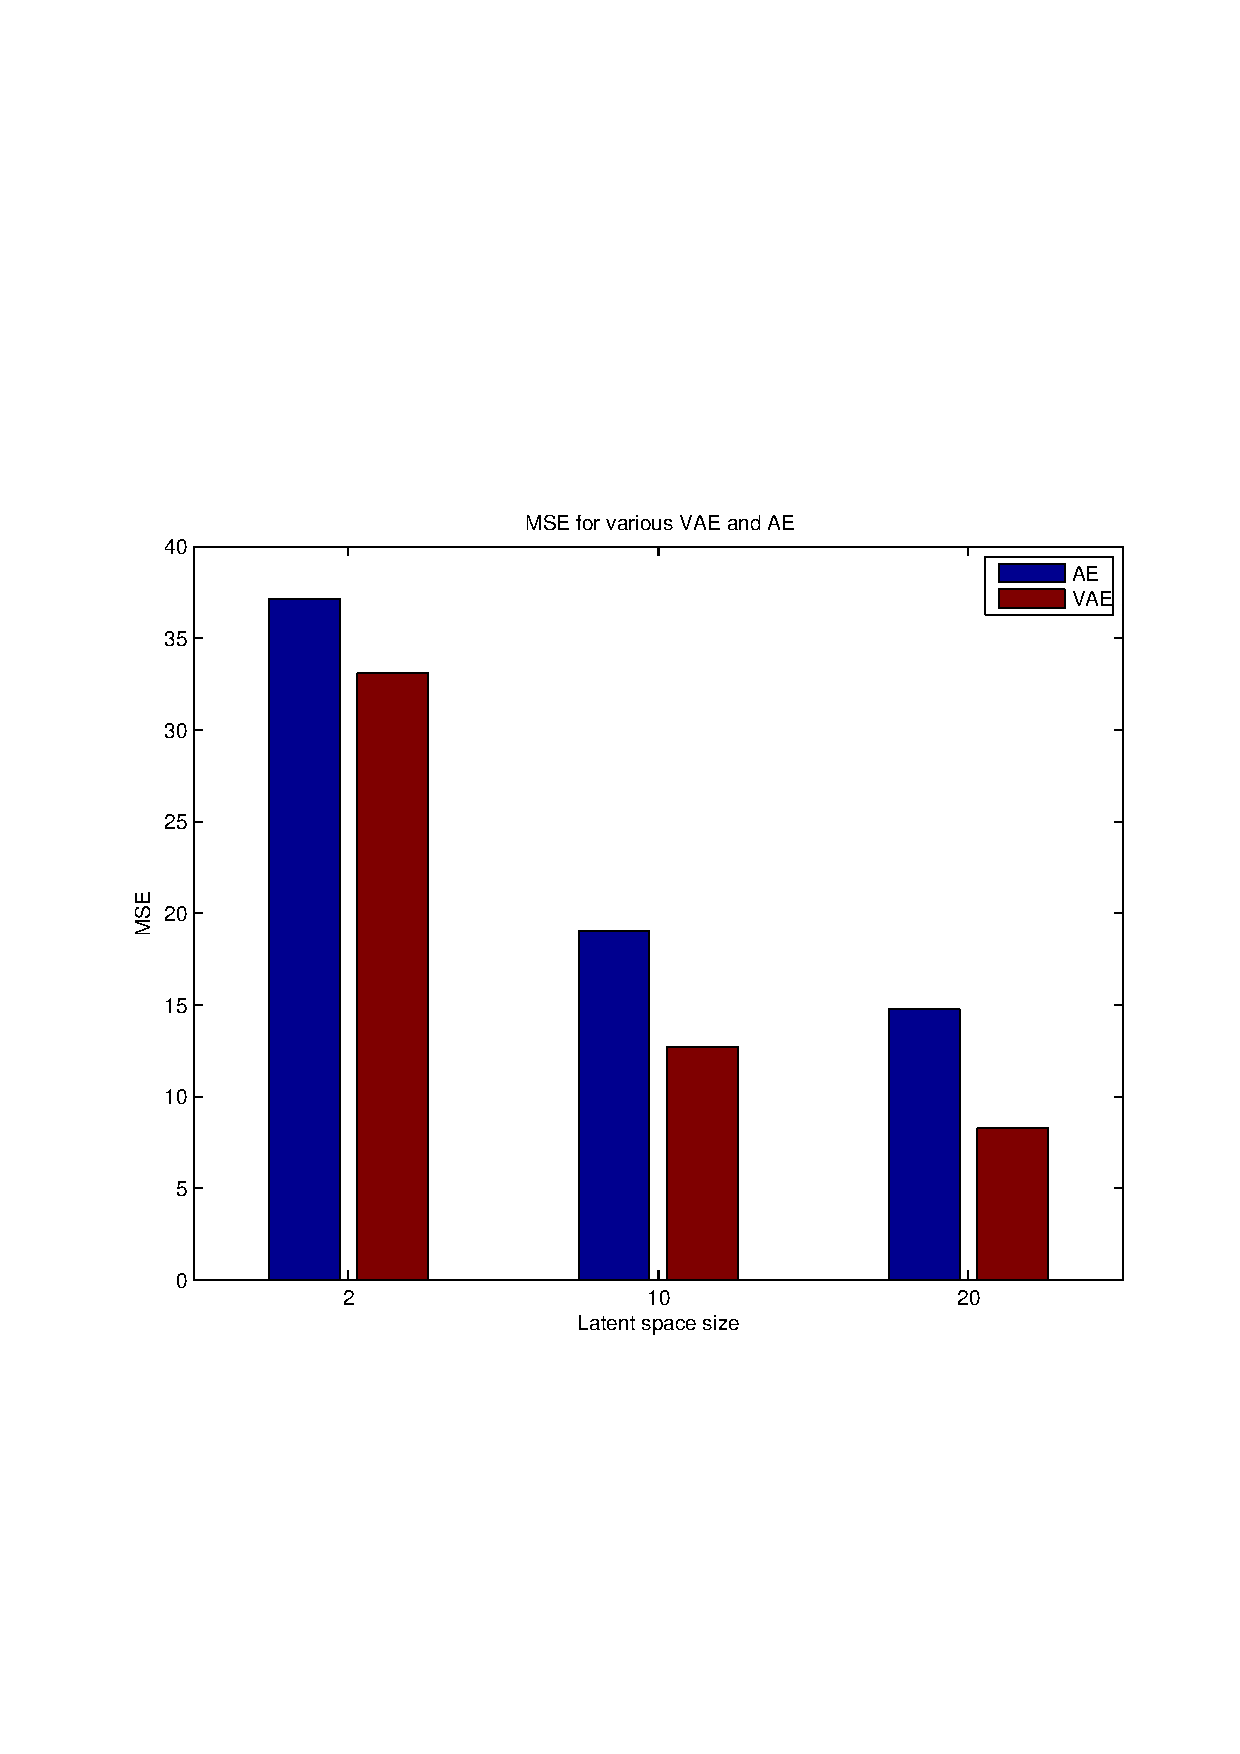
\includegraphics[width=0.8\columnwidth]{../res/mnist_mse.pdf}
\end{minipage} & 
\begin{minipage}[c]{0.5\columnwidth}
\begin{center}
\vspace{1.0cm}
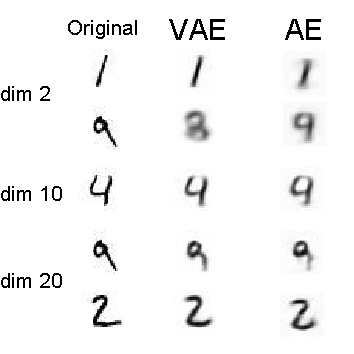
\includegraphics[width=.9\columnwidth]{../res/recon_mnist_compre.pdf}
\end{center}
\end{minipage}
\end{tabular}


\newpage %%%%%%%%%%%%%%%%%%%%%%%%%%%%%%%%%%%%%%%%%%%%%%%%%%%%%%%%%%%%%%%%%%%%%%%%%%%%%%%%%%%%%%%%%%%%%%%


\mysection{Full Variational Bayes}
Possible to perform full VB on parameters:
$$\mathcal{L}(\phi; \mathbf{X}) = \int q_\phi(\theta)(log\ p_\theta(X) + log\ p_\alpha(\theta) - log\ q_\phi(\theta)) d\theta$$
A differentiable Monte Carlo estimate to perform SGVB, yielding a distribution over parameters.\\
Implementation showed a decrease of variational lower bound, but no evidence of learning, possibly due to strict Gaussian assumptions of variational approximate posteriors.

\vspace{0.25in}

\mysection{Architecture experiments}

We examined various changes to the original architecture of the auto-encoder to test the robustness and flexibility of the model which lead to improvement in terms of optimising the lower bound and computational efficiency.

\begin{tabular}{cc}
\begin{minipage}[c]{0.25\columnwidth}
\begin{itemize}
\item Different activation functions.
\end{itemize}
\end{minipage} & 
\begin{minipage}[c]{0.75\columnwidth}
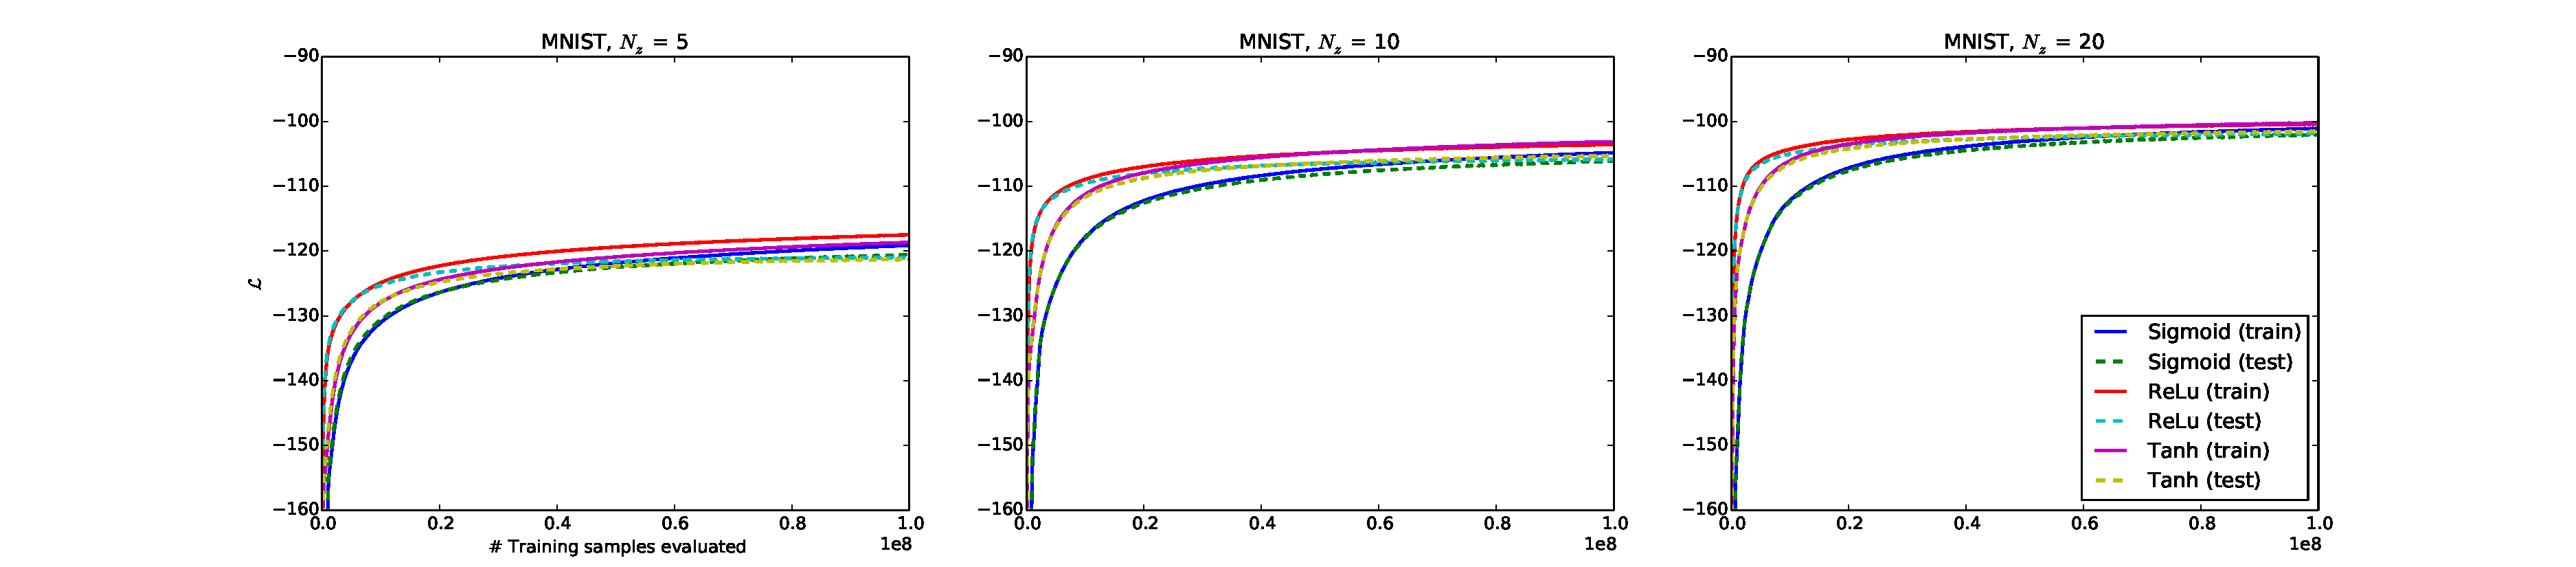
\includegraphics[width=1.0\columnwidth, clip, trim=4mm 0mm 4mm 4mm]{../res/mnist_activations}
\end{minipage}
\end{tabular}

\vspace{0.5em}

\begin{tabular}{cc}
\begin{minipage}[c]{0.25\columnwidth}
\begin{itemize}
\item Increasing the depth of the encoder.
\end{itemize}
\end{minipage} & 
\begin{minipage}[c]{0.75\columnwidth}
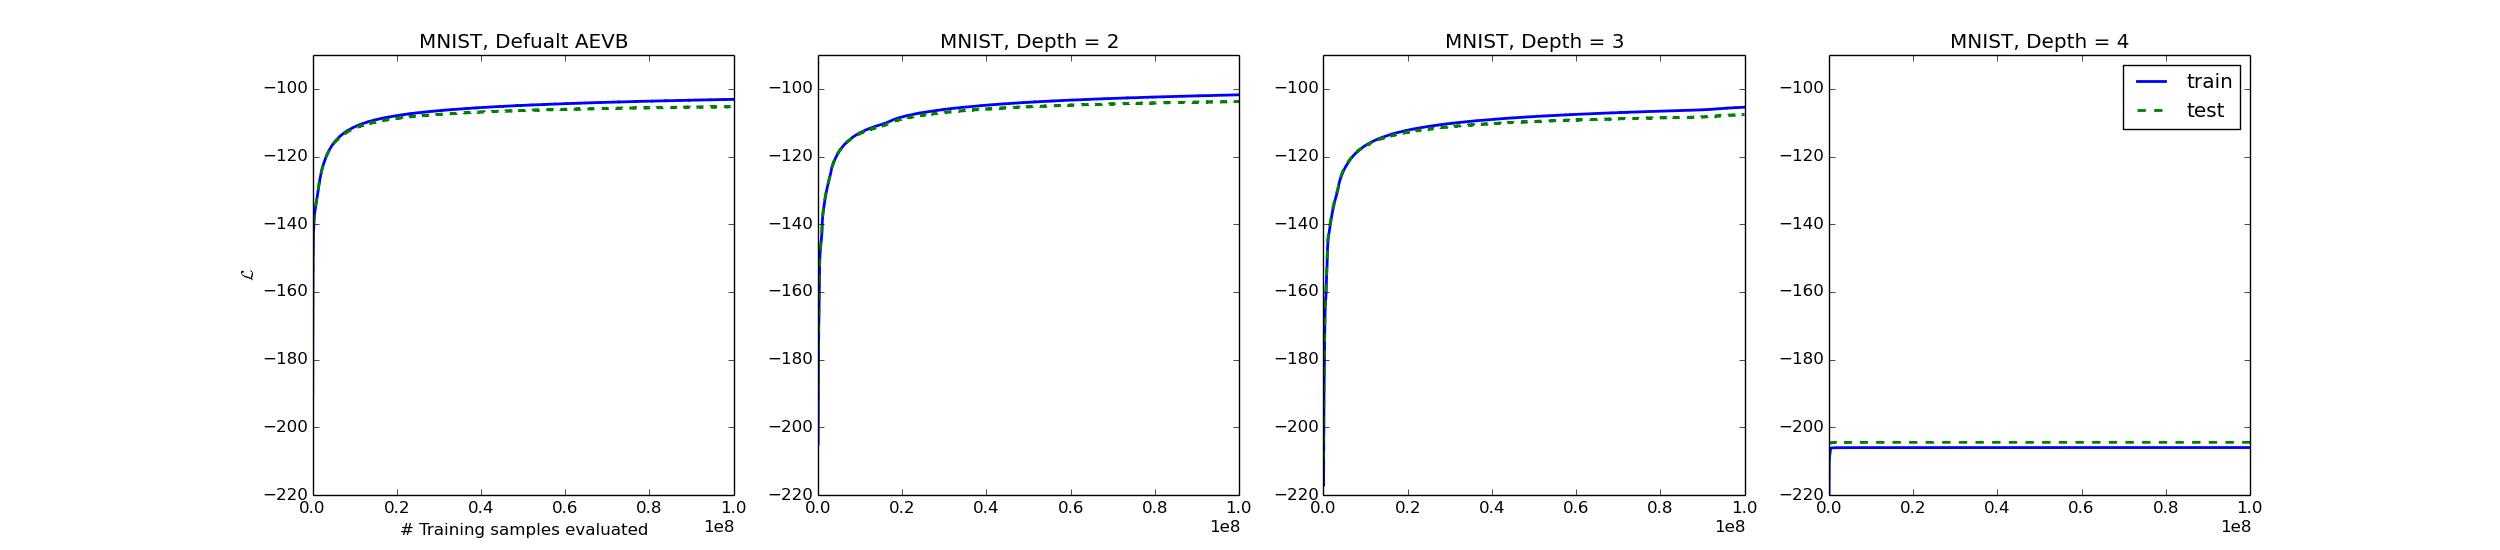
\includegraphics[width=1.0\columnwidth, clip, trim=4mm 0mm 4mm 4mm]{../res/mnist_depth}
\end{minipage}
\end{tabular}

\vspace{0.5em}

\mysection{Future works}
% enumerate doesnt seem to work here..
I.~~ Scheduled training of VAEB $[2]$.\\
II. ~~ Direct parameterization of differentiable transform $[3]$.\\
III. ~~ Different priors over latent space.
\vspace{0.5em}

\mysection{References}
\begin{enumerate}
\item Kingma, D. P., and  Welling M., "Auto-encoding variational bayes." arXiv preprint arXiv:1312.6114 (2013).
\item Geras, K. J., and Sutton C., "Scheduled denoising autoencoders." arXiv preprint arXiv:1406.3269 (2014).
\item Tran, D, Ranganath, R. and Blei, M. "Variational Gaussian Process" arXiv preprint arXiv:1511.06499 (2015).
\end{enumerate}

\end{multicols}
\end{poster}

\end{document}

